\documentclass{article}
\usepackage{amssymb}
\usepackage{amsmath}
\usepackage[utf8]{inputenc}
\usepackage{enumerate}

\title{Yet Another SAT Encoding for Car Sequencing} 
%\author{Valentin Mayer-Eichberger and Martin Gebser}

\usepackage{tikz}
\usetikzlibrary{arrows,shapes}
\usepackage{graphics}
\usepackage[showboxes]{textpos}

\def\qed{{\hfill $\Box$}}
\def\proof{{\noindent \textit{Proof.~}}}
\newtheorem{definition}{Definition}[section]
\newtheorem{lemma}{Lemma}[section]
\newtheorem{proposition}{Proposition}[section]
\newtheorem{theorem}{Theorem}[section]
\newtheorem{corollary}{Corollary}[section]
\newtheorem{example}{Example}[section]
\newtheorem{conjecture}{Conjecture}[section]

\def\constraint#1{\mbox{{\rm\sc #1}}}
\def\reachability{{\constraint{reachability }}}

%\def\edge{\operatorname{edge}}
%\def\reach{\operatorname{reach}}
%\def\path{\operatorname{path}}
%\def\start{\operatorname{start}}
%\def\stop{\operatorname{end}}
%\def\one#1{\constraint{Exactly1}(#1)}

\def\implies{\Rightarrow}
\def\when{\Leftarrow}
\def\and{\wedge}

\begin{document}

\maketitle

The encoding avoids a separate counter encoding for each cardinality
constraint and  at the same time is an alternative to \cite{Mayer13}. 

The encoding is wrt. one object (car or option) for which we omit the
subscript. We present an encoding for the constraint

$$\bigwedge_{i=0}^{n-q}(\sum_{l=1}^q x_{i+l} \leq u )$$

\begin{itemize}
    \item $x_i$ is true (1) if the object is at position $i$. 
    \item $s_{i,j}$ is true if in window $[i-q+1, \ldots i]$ there are at least $j$ objects. 
\end{itemize}

$$s_{i,j} \;\;\; \Leftrightarrow \;\;\; \sum_{l=i-q+1}^i x_l \geq j $$

The idea behind the clauses is to express the relationship between $x_{i-q}$,
$x_i$ and the counter $s_{i,j}$. 

\begin{align}
    \neg s_{i,j} & \vee s_{i+1,j-1} \\
    \neg s_{i+1,j} & \vee s_{i,j-1} \\
    \neg s_{i,j} & \vee s_{i,j-1} \\
    \neg x_i & \vee \neg s_{i-1,j} \vee s_{i,j} \\
         x_i & \vee \neg s_{i,j} \vee s_{i-1,j} \\
    \neg x_{i-q} & \vee \neg s_{i,j} \vee s_{i-1,j} \\
         x_{i-q} & \vee \neg s_{i-1,j} \vee s_{i,j} \\
    \neg x_i \vee x_{i-q} & \vee \neg s_{i-1,j-1} \vee s_{i,j} \\
         x_i \vee \neg x_{i-q} & \vee \neg s_{i,j-1} \vee s_{i-1,j}
\end{align}


\vspace{2cm}
\begin{center}

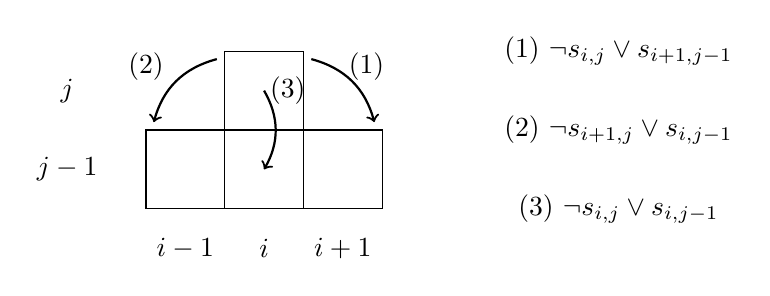
\begin{tikzpicture}[node distance=1cm, auto,]

\coordinate (A) at (0.1,1.1);
\coordinate (B) at (0.9,1.9);

\coordinate (C) at (2.1,1.9);
\coordinate (D) at (2.9,1.1);

\coordinate (E) at (1.5,1.5);
\coordinate (F) at (1.5,0.5);

\draw (0, 0) rectangle (1, 1);
\draw (1, 1) rectangle (2, 2);
\draw (1, 0) rectangle (2, 1);
\draw (2, 0) rectangle (3, 1);
\draw[->,thick] (B) to [bend right] (A);
\draw[->,thick] (C) to [bend left] (D);
\draw[->,thick] (E) to [bend left] (F);

%\node at (0.7,0.5) {$s_{i-1,j-1}$};
%\node at (1.5,1.5) {$s_{i,j}$};

\node at (-1,0.5) {$j-1$};
\node at (-1,1.5) {$j$};
\node at (0.5,-0.5) {$i-1$};
\node at (1.5,-0.5) {$i$};
\node at (2.5,-0.5) {$i+1$};

\node at (2.8,1.8) {$(1)$};
\node at (0,1.8) {$(2)$};
\node at (1.8,1.5) {$(3)$};
%\node at (2,0) {test};

\node at (6,2) {(1) $ \neg s_{i,j} \vee s_{i+1,j-1}$};
\node at (6,1) {(2) $ \neg s_{i+1,j} \vee s_{i,j-1}$};
\node at (6,0) {(3) $ \neg s_{i,j} \vee s_{i,j-1}$};

\end{tikzpicture}

\vspace{2cm}

\begin{tikzpicture}[node distance=1cm, auto,]

\coordinate (A) at (0.5,1.1);
\coordinate (B) at (1.5,1.1);

\coordinate (C) at (0.5,-0.1);
\coordinate (D) at (1.5,-0.1);


\draw (0, 0) rectangle (1, 1);
\draw (1, 0) rectangle (2, 1);
\draw[<->,thick] (A) to [bend left] (B);
%\draw[<->,thick] (C) to [bend right] (D);

\node at (-1,0.5) {$j$};
\node at (0.5,-0.6) {$i-1$};
\node at (1.5,-0.6) {$i$};

%\node at (2.8,1.8) {$(1)$};
%\node at (0,1.8) {$(2)$};
%\node at (1.8,1.5) {$(3)$};

\node at (6,3) {(4) $  \neg x_i  \vee \neg s_{i-1,j} \vee s_{i,j} $};
\node at (6,2) {(5) $       x_i  \vee \neg s_{i,j} \vee s_{i-1,j} $};
\node at (6,1) {(6) $  \neg x_{i-q}  \vee \neg s_{i,j} \vee s_{i-1,j} $};
\node at (6,0) {(7) $       x_{i-q}  \vee \neg s_{i-1,j} \vee s_{i,j} $};

\end{tikzpicture}

\vspace{2cm}
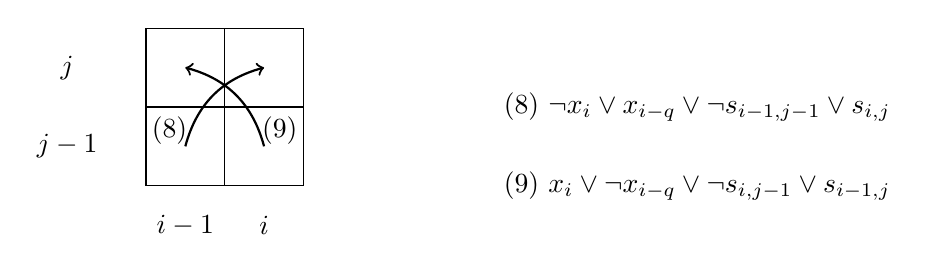
\begin{tikzpicture}[node distance=1cm, auto,]

\coordinate (A) at (0.5,0.5);
\coordinate (B) at (1.5,1.5);

\coordinate (C) at (0.5,1.5);
\coordinate (D) at (1.5,0.5);


\draw (0, 0) rectangle (1, 1);
\draw (1, 1) rectangle (2, 2);
\draw (1, 0) rectangle (2, 1);
\draw (0, 1) rectangle (1, 2);
\draw[->,thick] (A) to [bend left] (B);
\draw[->,thick] (D) to [bend right] (C);

\node at (-1,0.5) {$j-1$};
\node at (-1,1.5) {$j$};
\node at (0.5,-0.5) {$i-1$};
\node at (1.5,-0.5) {$i$};


\node at (0.3,0.7) {$(8)$};
\node at (1.7,0.7) {$(9)$};

\node at (7,1) {(8) $\neg x_i \vee x_{i-q} \vee \neg s_{i-1,j-1} \vee s_{i,j} $};
\node at (7,0) {(9) $ x_i \vee \neg x_{i-q} \vee \neg s_{i,j-1} \vee s_{i-1,j}$};

\end{tikzpicture}


\end{center}


\bibliographystyle{plain}
\bibliography{p}

\end{document}
